\documentclass[aspectratio=1610]{beamer}
 
\usepackage[utf8]{inputenc}
\usepackage{hyperref}
 
\title{Exploring the provision of online booter services}
\author{Paper by Dr Alice Hutchings and Dr Richard Clayton}
\institute{Presented by Chongyang Shi}
\date{November 13, 2017}
 
\begin{document}
 
\frame{\titlepage}
 
% Historical context
 
\begin{frame}
\frametitle{Historical Context: Booter Services}
\begin{itemize}
\setlength\itemsep{1em}
\item Distributed Denial of Service (DDoS) attacks have been around since late last century. (Yan et al., 2000) \cite{yan2000xenoservice}
\item Booters are low-cost short-duration DDoS attacks sold as a service, with their name coined by Karami and McCoy in 2013. \cite{karami2013understanding}
\item Often used for petty reasons such as disrupting an online gaming opponent. \cite[p. 1163]{hutchings2016exploring}
\item Provisioning and use are illegal under Computer Misuse Act 1990 and others.

\end{itemize}
\end{frame}

\begin{frame}
\frametitle{Historical Context: Assessing the Scale of Operations}
Leaked database from a single operator: \par
\begin{itemize}
\setlength\itemsep{1em}
\item48,000 attacks, 11,000 victims over 52 days, yielding US\$7,727 per month. 
\item Most users were gamers using short attacks up to 10 minutes.
\end{itemize}
\vspace{1em}
While the technical methods behind these services have been studied in detail \cite{karami2013understanding}, the scales and motivations of their operators had not been studied.
\begin{itemize}
\setlength\itemsep{1em}
\item The need for a more comprehensive study into the booter service ``industry".
\item There have been few research into cybercrime offenders themselves overall. \cite{holt2014assessment}
\end{itemize}
\end{frame}

% Technical concepts
\begin{frame}
\frametitle{Key Definition: DDoS Attacks}
\begin{itemize}
\setlength\itemsep{1em}
\item DDoS attacks seek to prevent legitimate access to the victim server by sending an overwhelming amount of requests.
\item DDoS attacks can be amplified by forging packet headers to achieve reflection.
\item Reflected attacks cost less to initiate and cost more to filter -- vastly favouring the attacker.
\item Reflector attacks exploit the unauthenticated nature of common protocols.
\item Other types of attacks also seen offered by booter services, such as HTTP flood on Layer 7, but far less ``efficient".
\end{itemize}
\end{frame}

% Criminology concepts

\begin{frame}
\frametitle{Key Definition: Criminology Theories}
Traditional criminology theories will be used to study booter service operators: \par
\vspace{0.5em}
\begin{itemize}
\setlength\itemsep{1em}
\item Differential association
\item Techniques of neutralisation
\item Rational choice theory
\end{itemize}
\end{frame}

\begin{frame}
\frametitle{Key Definition: Differential Association}
Sutherland's theory of differential association \cite{sutherland1983white}: \par
\begin{itemize}
\setlength\itemsep{1em}
\item Criminal behaviour is normal behaviour learnt in interaction with others in intimate personal groups.
\item Different people respond to criminal behaviours of peers differently. Response also dependent on frequency of association.
\item Online communities have made differential association easier for cybercrime offenders.
\item Demographic features of these communities.
\item Greater the differential association, greater the likelihood of self-reporting their participation.
\end{itemize}
\end{frame}

\begin{frame}
\frametitle{Key Definition: Techniques of Neutralisation}
Sykes and Matza's theory on techniques of neutralisation \cite{sykes1957techniques}: \par
\begin{itemize}
\setlength\itemsep{1em}
\item Offenders learn to use techniques to justify or neutralise acts to mitigate feelings of shame or guilt.
\item Offenders may distinguish between ``appropriate and inappropriate" targets.
\item Techniques include denying responsibility, injury or victims; condemning the condemners; appealing to higher loyalties.  
\item Computer as a medium makes neutralisation easier.
\item Some techniques more frequently observed in cybercrime offenders than others.
\end{itemize}
\end{frame}

\begin{frame}
\frametitle{Key Definition: Rational Choice Theory}
Cornish and Clarke's theory of rational choice \cite{cornish1987understanding}: \par
\begin{itemize}
\setlength\itemsep{1em}
\item Offenders calculate the perceived cost and benefits of crime, in seeking some kind of advantage.
\item Offenders assess their skills and resources against perceived risk.
\item Risk of detection and risk of punishment may bear different weights.
\item Cybercrime: usually low perceived risk, benefits primarily financial.
\item Personal gratification gained from committing skilled crimes.
\end{itemize}
\end{frame}

% The study described

\begin{frame}
\frametitle{The Study: Overview}
\begin{itemize}
\setlength\itemsep{1em}
\item Conducted from July to September 2014.
\item Mixed method and cross-sectional design.
\item Attempt to examine the entire population of booter service operators.
\item Data analysed with quantitative (limited due to sample size) and qualitative analysis. 
\end{itemize}
\end{frame}

\begin{frame}
\frametitle{Results: Recruiting Participants}
\begin{quote}
How the f--- did you get to it? I don't even advertise it anywhere and have no idea how you even found it.
\end{quote}
\begin{flushright} A booter service operator participating anonymously in the study \end{flushright} 
\end{frame}

\begin{frame}
\frametitle{The Study: Recruiting Participants}
\begin{itemize}
\setlength\itemsep{1em}
\item Focused on openly advertised operators only, operators in hidden services not surveyed.
\item Keyword search, online criminal forums.
\item Collection process conducted more than once to find more operators.
\item Some booter services may be operated by the same operator.
\item Operators contacted via public/customer contact information.
\end{itemize}
\end{frame}

\begin{frame}
\frametitle{The Study: Conducting the Survey}
\begin{itemize}
\setlength\itemsep{1em}
\item Aim of study explained to the contacted operators.
\item Randomised invitations to either an online survey or an interactive interview.
\item Alternative participation method sent if no response.
\item 63 invited, 13 responses (from 12 unique sites), 11 completed the survey, while 2 were interviewed.
\item Overall response rate 25\%, higher than expected. 
\end{itemize}
\end{frame}


\begin{frame}
\frametitle{The Study: Purpose of the Survey}
The survey aims to understand: \par
\begin{itemize}
\setlength\itemsep{1em}
\item Motivations of booter service operators.
\item Perceptions of legality in operating booter services.
\item Market and economic benefits.
\item Time commitment, reasons for involvement, methods of involvement.
\item Technical aspects of their services.
\end{itemize}
\vspace{0.5em}
All questions were optional to encourage involvement.
\end{frame}

% Results w.r.t participant demographics

\begin{frame}
\frametitle{Results: Participant Characteristics}
\begin{quote}
Because in the future I don't plan on having a job so shitty that I need to resort to reviewing f------ booters. 
\end{quote}
\begin{flushright} A booter service operator when asked about future aspirations \end{flushright} 
\end{frame}

\begin{frame}
\frametitle{Results: Participant Characteristics}
General demographics of participants: \par
\begin{itemize}
\setlength\itemsep{1em}
\item Barring creative responses, it is apparent that all participants are male. 
\item All between 16 and 34 years old.
\item Most operated a booter service for less than 3 years.
\item From 5 different continents.
\item Mostly student, but also include two with other employments.
\end{itemize}
\end{frame}

\begin{frame}
\frametitle{Results: Participant Characteristics}
\begin{itemize}
\setlength\itemsep{1em}
\item Most operators consider themselves to have a high level of technical proficiency.
\item Originating from related skills such as web development and OS/networks knowledge.
\item Some have a gradual pathway to offending, starting as a user of these services.
\item Some provide backbone services to other booter service operators.
\item Many operators also operate other online services, both legal and illegal.
\end{itemize}
\end{frame}

% Results w.r.t criminology aspects

\begin{frame}
\frametitle{Results: Differential Association Analysis}
\begin{itemize}
\setlength\itemsep{1em}
\item Booter service operators often start offending under the influence of others, or through exposure to these services via gaming and online communities.
\item Some had peers already in the business, and were introduced to profit potentials.
\item Learning technical skills and providing legitimate pentest tools were also motivations.
\end{itemize}
\end{frame}

\begin{frame}
\frametitle{Results: Techniques of Neutralisation}
\begin{itemize}
\setlength\itemsep{1em}
\item Majority of operators surveyed attempted to neutralise or excuse their behaviour.
\item Appealing to higher loyalties: providing service ``for the common good'' to create more secure systems overall.
\item Perceptions of legality: some operators believe that booter services are not illegal in their jurisdiction, or vary by target of attack.
\item Denying responsibility: some believe that the users of their services are responsible for using it for purposes other than stressing their own networks.
\item Condemning the condemner: one participants questions the severity of booter services when compared with online pornography and other illegal activities.  
\end{itemize}
\end{frame}

\begin{frame}
\frametitle{Results: Techniques of Neutralisation}
\begin{itemize}
\setlength\itemsep{1em}
\item Cross-comparison of responses also reveal interesting observations.
\item Booter service operators consider the use of their services against different types of targets differ in legality and moral correctness.
\item In denying responsibility, many booter service operators believe that it would be illegal to use their services against third-party targets, but it will not be up to them to police it, echoing appeals to higher loyalties.
\end{itemize}
\vspace{-5em}
\begin{figure}
\centering
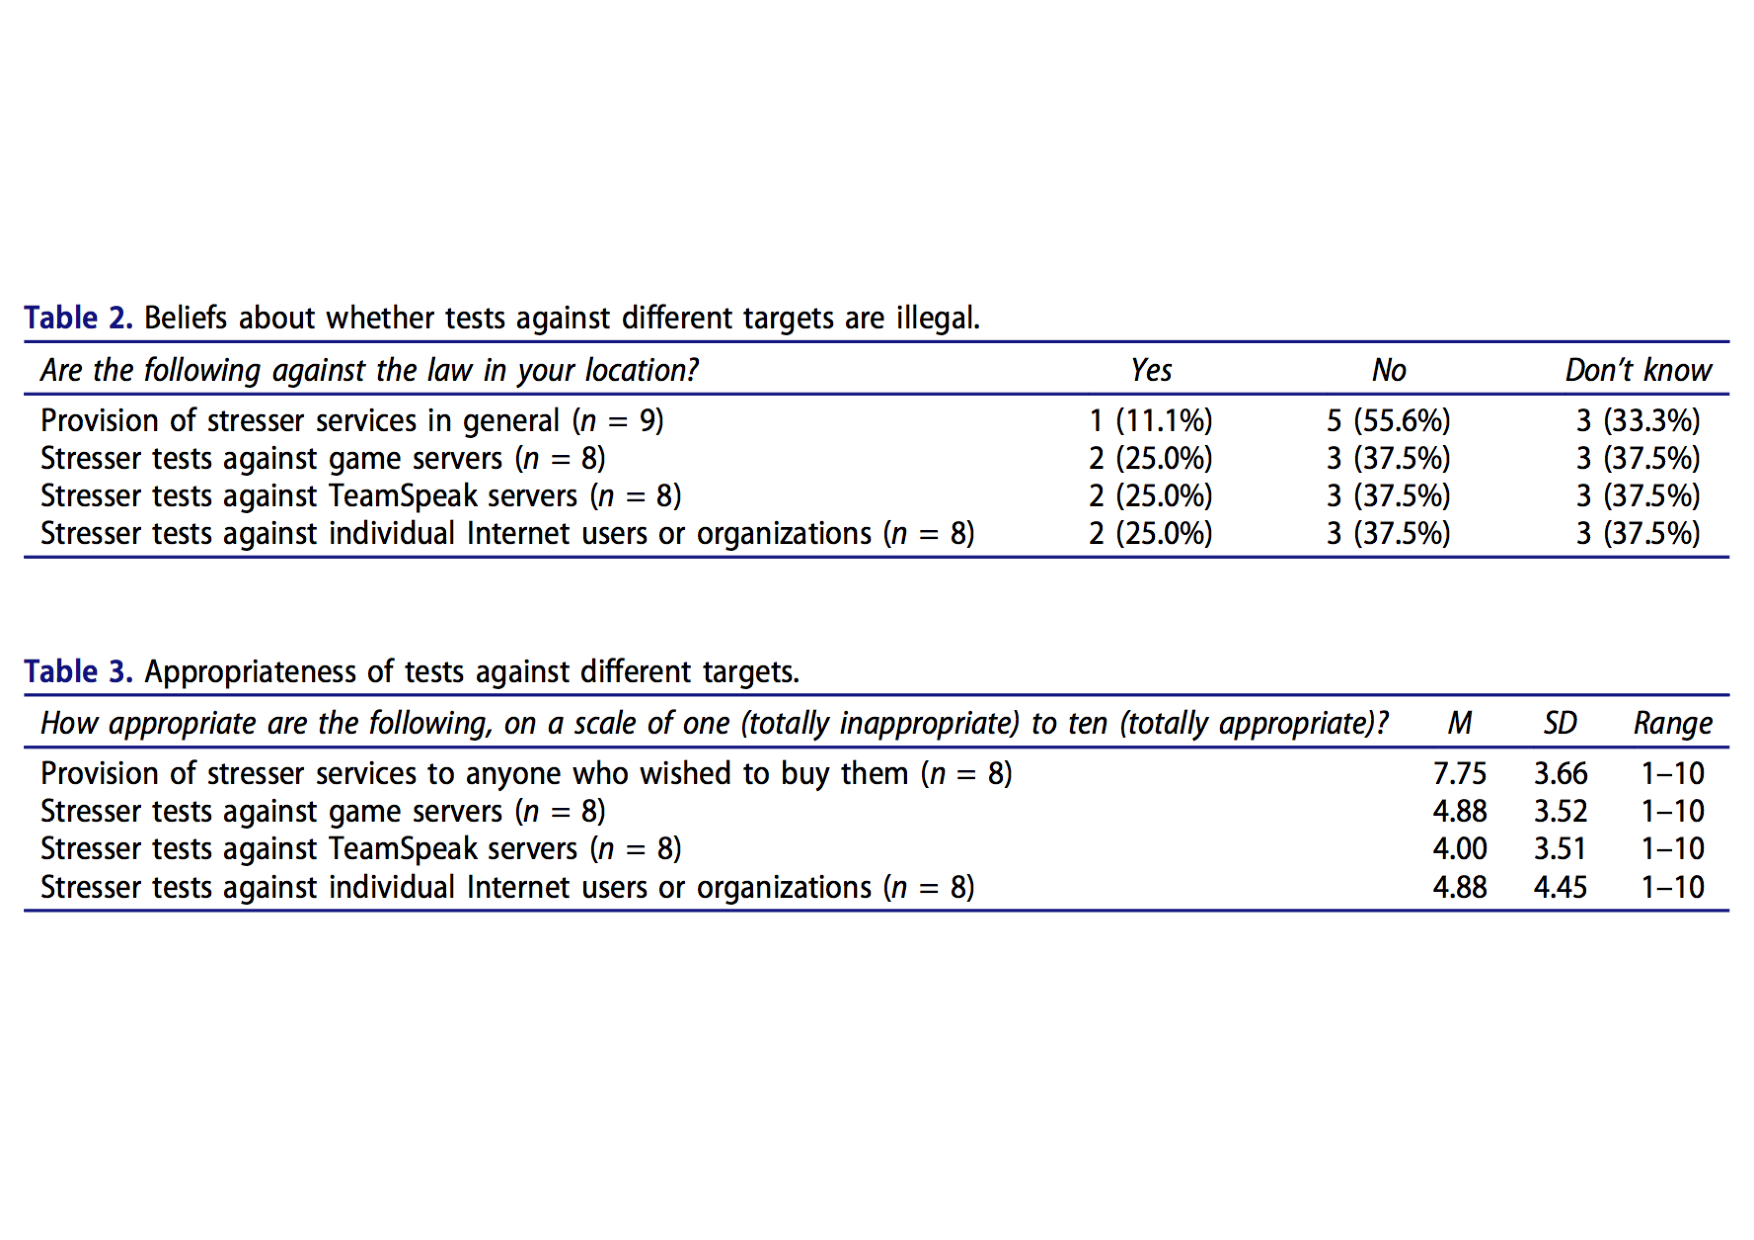
\includegraphics[scale=0.4]{fig1.pdf}
\end{figure}
\end{frame}

\begin{frame}
\frametitle{Results: Rational Choice analysis}
\begin{itemize}
\setlength\itemsep{1em}
\item Financial gains appear to be the prime motivation for booter service operators.
\item Conservative estimate of income is between US\$3705.25 and US\$5430.67.
\item However, it is not a significant income source to all operators, the responses were evenly distributed.
\item Operators invest vastly different amounts of time into maintaining their service.
\item Technical excitement is also a motivation to some operators.
\end{itemize}
\end{frame}

\begin{frame}
\frametitle{Results: Service Architecture}
\begin{itemize}
\setlength\itemsep{1em}
\item Both Layer 3/4 and Layer 7 DDoS attacks offered by operators.
\item Generally moving away from Layer 7 due to increased accessibility of DDoS protection products.
\item Technically proficient operators programmed their own systems, while others paid for others to code.
\item Some operators run services on their own, others have collaborators.
\item Search engine and URL access are primary methods of reaching the services. 
\end{itemize}
\end{frame}

\begin{frame}
\frametitle{Results: Attack Targets}
\vspace{1em}
Aggregated percentages of attack targets: \par
\begin{figure}
\centering
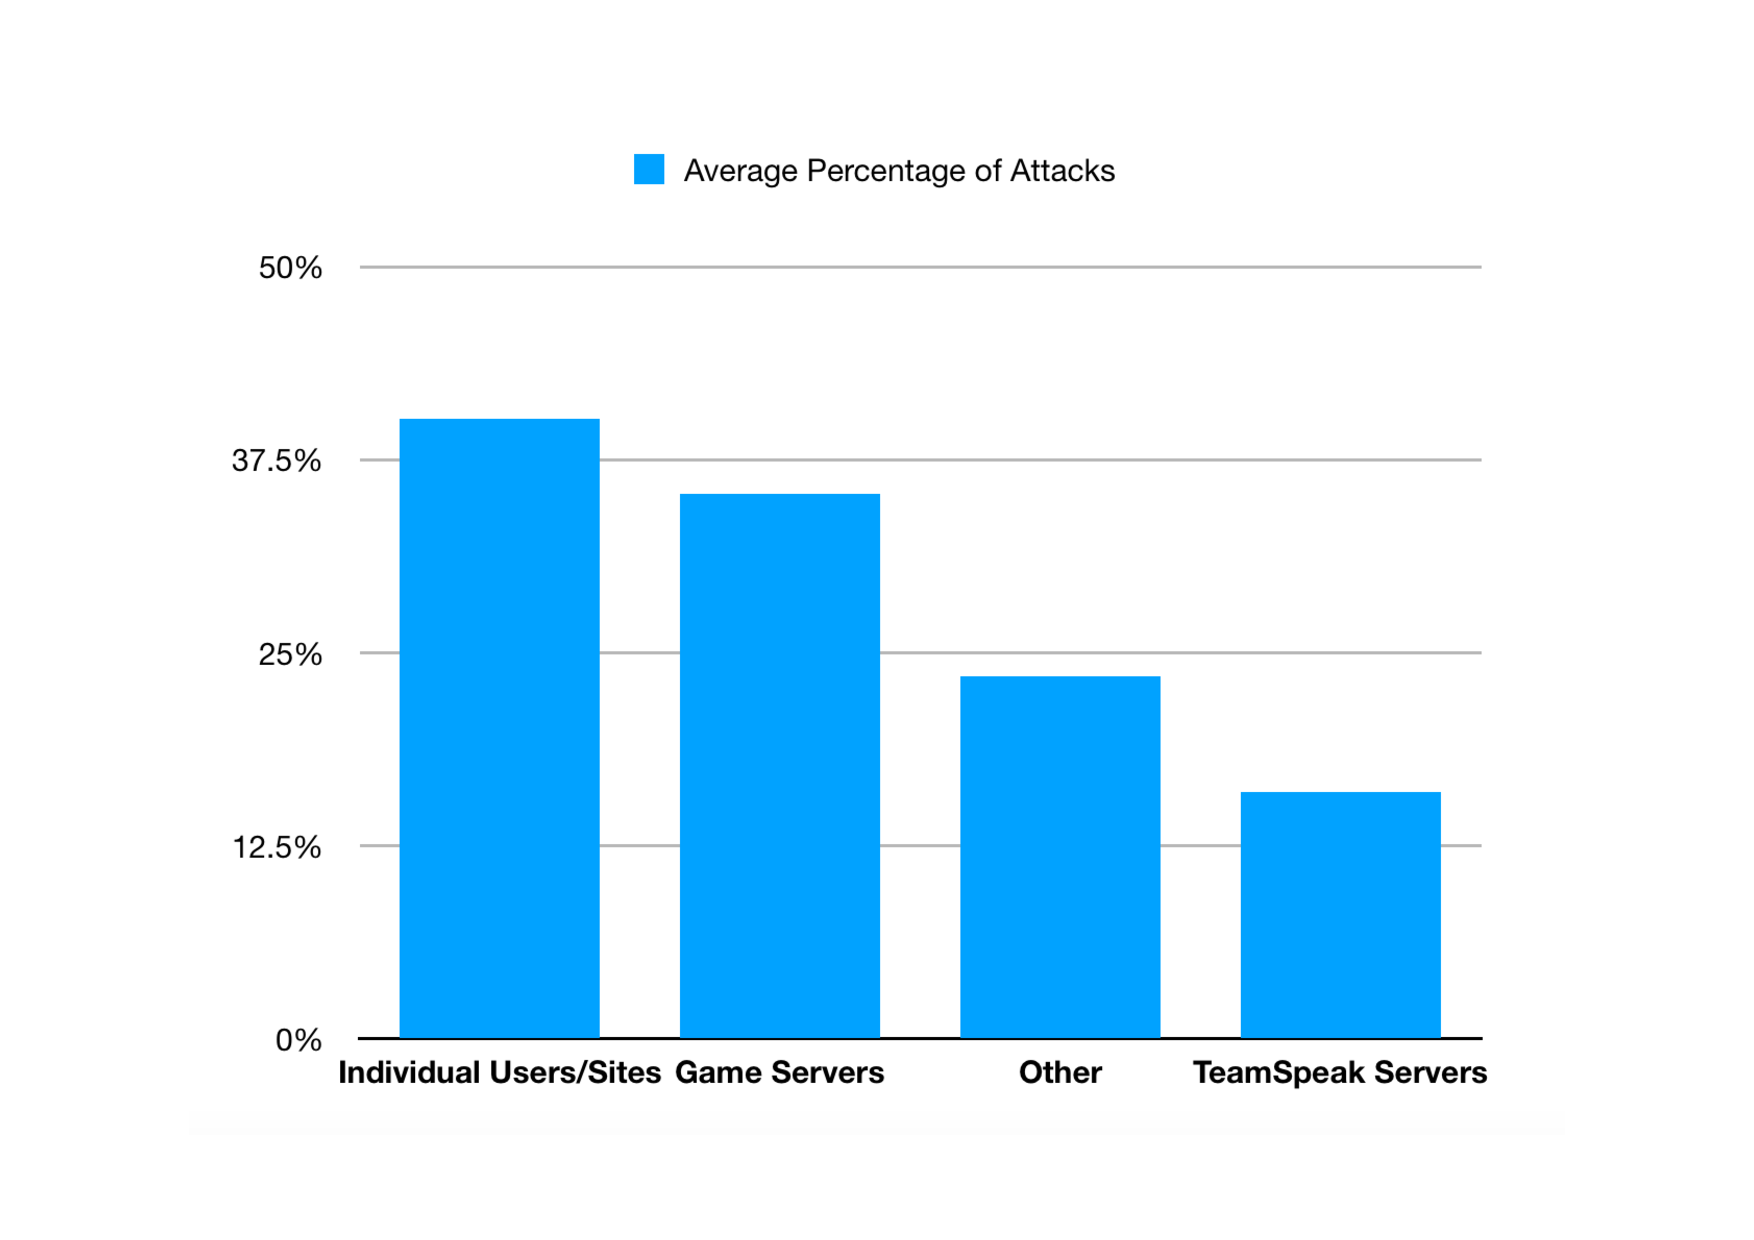
\includegraphics[scale=0.4]{fig2.pdf}
\end{figure}
\end{frame}

% Papers cited

\begin{frame}
\frametitle{Selected Cited Papers}
Prior analysis of Booter services, mostly on technical aspects: \par
\begin{itemize}
\item \emph{Understanding the Emerging Threat of DDoS-as-a-Service}, Karami and McCoy, 2013 \cite{karami2013understanding}
\item \emph{Rent to Pwn: Analyzing Commodity Booter DDoS Services}, Karami and McCoy, 2013 \cite{karami2013rent}
\item \emph{Characterizing and mitigating the DDoS-as-a-service phenomenon}, Santanna and Sperotto, 2014 \cite{santanna2014characterizing}
\end{itemize}
\vspace{0.5em}
Criminology theories used: \par
\begin{itemize}
\item Differential association: Sutherland, 1949  \cite{sutherland1983white}
\item Techniques of neutralisation: Sykes and Matza, 1957 \cite{sykes1957techniques}
\item Rational choice theory: Cornish and Clarke, 1987 \cite{cornish1987understanding}
\end{itemize}
Several of the authors' previous works are also ingrained in the criminology analysis.
\end{frame}

% Related/current context

\begin{frame}
\frametitle{Current Context}
Characteristics of Booter victims (primarily residential users, content popularity has little effect): \par
\emph{Who gets the boot? Analyzing victimization by DDoS-as-a-Service} A. Noroozian et al., 2016 \cite{noroozian2016gets} \par
\vspace{1em}
Automatic identification of Booter services (identifying more potential booter services with crawling): \par
\emph{Booter blacklist: Unveiling DDoS-for-hire websites}, J. J. Santanna et al., 2016 \cite{santanna2016booter} \par
\vspace{1em}
Collecting research data from illicit sources:\par
\emph{Ethical issues in research using datasets of illicit origin}, D. R. Thomas et al., 2017 \cite{thomas2017ethical} 
\end{frame}

% Critique 

\begin{frame}
\frametitle{Critique}
Owing to the illicit nature of the services studied, the limited sample size makes ascertaining the conclusions difficult:
\begin{itemize}
\vspace{1em}
\item Sample size
	\begin{itemize}
	\item 63 services manually identified, 13 responses, most questions not answered by all participants.
	\item Deriving statistically significant data is difficult.
	\item Could automatic booter service identification \cite{santanna2016booter} help?  
	\end{itemize}
\vspace{1em}
\item Sample coverage
	\begin{itemize}
	\item While most booter services are openly advertised, would it be possible to assess the scale of their operations on hidden services (``the dark web'')?
	\item All participants operate in English, would the characteristics of operations of non-English booter services differ?
	\item As identified by the authors, the self-selection bias may affect responses used in criminology analysis.
	\end{itemize}
\end{itemize}

\end{frame}

% Suggestions for discussion

\begin{frame}
\frametitle{Suggested Discussions}
\begin{itemize}
\setlength\itemsep{1em}
\item Are there ways to understand the motivations of illicit service operators while avoiding the self-selection bias inevitable resulted by surveying them?
\item To control the growth of booter services, what technical solutions are available to increase the perceived risk of operating booter services, or to reduce differential association of these communities?
\end{itemize}
\end{frame}

\begin{frame}[t, allowframebreaks]
\frametitle{References}
\bibliographystyle{IEEEtran}
\bibliography{presentation}
\end{frame}
 
\end{document}